\documentclass[conference]{IEEEtran}
% The preceding line is only needed to identify funding in the first footnote. If that is unneeded, please comment it out.
\usepackage{amsmath,amssymb,amsfonts}
\usepackage{algorithm2e}
\RestyleAlgo{ruled}
\usepackage{graphicx}
\usepackage{textcomp}
\usepackage{xcolor}
\usepackage{subcaption}
\usepackage{booktabs}
\usepackage{tabularx}
\usepackage{multirow}
\usepackage[style=numeric,sorting=none]{biblatex}
\addbibresource{reference.bib}
\def\BibTeX{{\rm B\kern-.05em{\sc i\kern-.025em b}\kern-.08em
    T\kern-.1667em\lower.7ex\hbox{E}\kern-.125emX}}
\begin{document}

\title{A Genetic Simulated Annealing Algorithm for the Capacitated Arc Routing Problem}

\author{
    \IEEEauthorblockN{Mengxuan Wu}
    \IEEEauthorblockA{
        \textit{Department of Computer Science and Engineering} \\
        \textit{Southern University of Science and Technology} \\
        12212006@mail.sustech.edu.cn
    }
}

\maketitle

\begin{abstract}
    The Capacitated Arc Routing Problem (CARP) is a combinatorial optimization problem that is NP-hard. 
    In this paper, we propose a Genetic Simulated Annealing Algorithm to solve the CARP. 
    The algorithm uses simulated annealing to explore the solution space and genetic algorithms to maintain a population of potential solutions.
    In addition to the basic move operators, we also incorporate a new move operator called the Merge-Split operator introduced by Yi Mei et al. \cite{MEANS}.
    The algorithm is then tested on the various benchmark instances of the CARP.
\end{abstract}

\section{Introduction}
\label{sec:introduction}

The Capacitated Arc Routing Problem (CARP), which is one form of the Arc Routing Problem (ARP), is a combinatorial optimization problem.
It is first introduced by Golden et al. \cite{CARP} in 1984.
Unlike the Vehicle Routing Problem (VRP), the CARP serves customers on arcs instead of nodes.
The problem can be briefly described as follows: 
\begin{enumerate}
    \item Given a graph $G = (V, E)$, and a set of arcs $A \subseteq E$. 
        Each arc $a \in A$ has a demand $q_a$, and each edge $e \in E$ has a cost $c_e$.
    \item A fleet of vehicles with a capacity $Q$ is available.
    \item Each route starts and ends at the depot, and the total demand of each route does not exceed the capacity of the vehicle.
    \item The objective is to find a set of routes that minimizes the total cost of the routes.
\end{enumerate}

It is evident that the CARP has many real-world applications, such as garbage collection, street sweeping, and snow removal.
However, the CARP is NP-hard, which means that it is difficult to find an exact solution in a reasonable amount of time.
Therefore, many heuristic and metaheuristic algorithms have been proposed to solve the CARP.
Representative heuristic algorithms include Path-Scanning \cite{CARP}, Augmenting Path \cite{Augment-insert}, Ulusoy's Route First-Cluster Second, etc.
Representative metaheuristic algorithms include Memetic Algorithm (MA) \cite{Lacomme2004Competitive}, Genetic Algorithm (GA) \cite{Lacomme2001A}, Variable Neighborhood Search (VNS) \cite{Hertz2001A}, etc.

In this paper, we propose a Genetic Simulated Annealing Algorithm (GSA) to solve the CARP.
The algorithm uses simulated annealing with move operators to explore the solution space.
A genetic algorithm is used to maintain a population of diverse solutions and to guide the search process.
In addition to the basic move operators, we also incorporate a new move operator called the Merge-Split operator introduced by Yi Mei et al. \cite{MEANS}.

The rest of the paper is organized as follows.
Section \ref{sec:preliminary} formally defines the CARP.
Section \ref{sec:methodology} describes the proposed algorithm in detail.
Section \ref{sec:experiments} presents the experimental setup and results.
Finally, Section \ref{sec:conclusion} concludes the paper.

\section{Preliminary}
\label{sec:preliminary}

The Capacitated Arc Routing Problem (CARP) can be formally defined as follows.
A solution $s$ to the CARP is represented as a set of routes $s = \{R_1, R_2, \ldots, R_m\}$.
Each route $R_i$ is represented as a sequence of tasks $R_i = \{\tau_{i 1}, \tau_{i 2}, \ldots, \tau_{i l_i}\}$, where $\tau_{i j} \in T$ is a task and $l_i$ is the number of tasks in route $R_i$.
Attributes of task are: beginning vertex of task $\tau_{i j}$ as $head(\tau_{i j})$, ending vertex of task $\tau_{i j}$ as $tail(\tau_{i j})$, demand of task $\tau_{i j}$ as $d(\tau_{i j})$, and cost of task $\tau_{i j}$ as $c(\tau_{i j})$.
The depot is represented as $0$.
The cost of the shortest path between two vertices $i$ and $j$ is denoted as $pc(i, j)$.

The constraints of the CARP are as follows:
\begin{equation}
    \label{eq:1}
    \sum_{k=1}^{m} l_k = |T|
\end{equation}

\begin{equation}
    \label{eq:2}
    \tau_{i_1 j_1} \neq \tau_{i_2 j_2}, \forall (i_1, j_1 \neq i_2, j_2)
\end{equation}

\begin{equation}
    \label{eq:3}
    \tau_{i_1 j_1} \neq inv(\tau_{i_2 j_2}), \forall (i_1, j_1 \neq i_2, j_2)
\end{equation}

\begin{equation}
    \label{eq:4}
    \sum_{i=1}^{l_k} d(\tau_{k j}) \leq Q, \forall k
\end{equation}

\begin{equation}
    \label{eq:5}
    \tau_{i j} \in T
\end{equation}

To explain the constraints, Equation \ref{eq:1}, \ref{eq:2}, and \ref{eq:3} ensure that each task is assigned to exactly one route.
Equation \ref{eq:4} ensures that the demand of each route does not exceed the capacity of the vehicle.
Equation \ref{eq:5} defines the set of tasks.

The objective function of the CARP is to minimize the total cost of the routes, which is $TC(s)$ defined as follows:
\begin{equation}
    \label{eq:6}
    TC(s) = \sum_{k=1}^{m} RC(R_k)
\end{equation}
where $RC(R_k)$ is the cost of route $R_k$ defined as follows:
\begin{equation}
    \label{eq:7}
    \begin{split}
        RC(R_k) &= \sum_{i=1}^{l_k} c(\tau_{k i}) + pc(0, head(\tau_{k 1})) + pc(tail(\tau_{k l_k}), 0)\\
                &+ \sum_{i=2}^{l_k} pc(tail(\tau_{k i-1}), head(\tau_{k i}))
    \end{split}
\end{equation}

\section{Methodology}
\label{sec:methodology}

\subsection{General Workflow}

The proposed Genetic Simulated Annealing Algorithm (GSA) is a hybrid algorithm that combines simulated annealing and genetic algorithms.
The general workflow of the algorithm is as follows:
\begin{enumerate}
    \item Initialize the population with heuristic solutions.
    \item For each individual in the population, apply simulated annealing with move operators to explore the solution space.
    \item Select the best individuals from parent population and offspring population.
    \item If the stopping criterion is met, return the best individual, otherwise go to step 2.
\end{enumerate}

\begin{figure}[h]
    \centering
    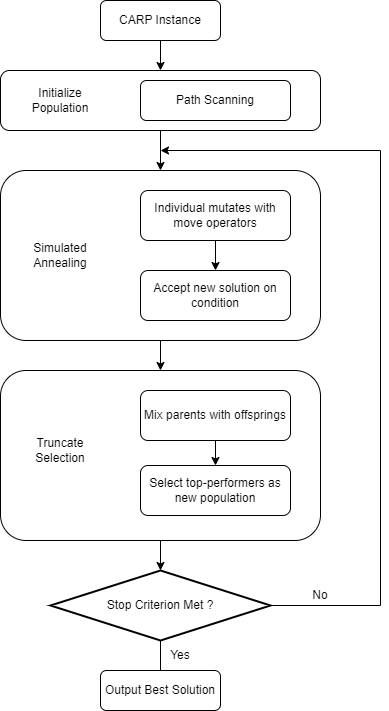
\includegraphics[width=0.35\textwidth]{flow chart.png}
    \caption{General workflow of the proposed algorithm}
    \label{fig:flowchart}
\end{figure}

\subsection{Detailed Implementation} 

\subsubsection{Initialization}

For the initialization of the population, we use the Path-Scanning algorithm \cite{CARP} to generate a set of feasible solutions.
The Path-Scanning algorithm is a simple and effective heuristic algorithm for the CARP.
It starts with an empty route and iteratively adds the nearest serviceable task to the route, until the capacity of the vehicle can no longer accommodate any remaining tasks.
The algorithm then starts a new route and repeats the process until all tasks are assigned to routes.
If multiple tasks are equidistant, the algorithm selects the task with one of the following strategies:
\begin{enumerate}
    \item The task closest to the depot.
    \item The task farthest from the depot.
    \item The task with the smallest demand-cost ratio.
    \item The task with the largest demand-cost ratio.
    \item If less than half of the capacity is used, used rule 1. Otherwise, use rule 2.
\end{enumerate}

\begin{algorithm}
    \caption{Path-Scanning Algorithm}
    \KwIn{A set of tasks $T$, a capacity $Q$}
    \KwOut{A set of routes $R$}
    $R \leftarrow \emptyset$\;
    $r \leftarrow \{(depot, depot)\}$\;
    $d_{cur} \leftarrow 0$\;
    \While{$T \neq \emptyset$}{
        $dist_{min} \leftarrow \infty$\;
        $t_{min} \leftarrow \emptyset$\;
        $t_{prev} \leftarrow r.last()$\;
        \ForEach{$\tau \in T$}{
            $dist \leftarrow pc(tail(t_{prev}), head(\tau))$\;
            \If{$dist < dist_{min}$ and $d_{cur} + d(\tau) \leq Q$}{
                $dist_{min} \leftarrow dist$\;
                $t_{min} \leftarrow \tau$\;
            }
        }
        \eIf{$t_{min} = \emptyset$}{
            $R \leftarrow R \cup \{r\}$\;
            $r \leftarrow \{(depot, depot)\}$\;
            $d_{cur} \leftarrow 0$\;
        }{
            $r \leftarrow r \cup \{t_{min}\}$\;
            $d_{cur} \leftarrow d_{cur} + d(t_{min})$\;
            $T \leftarrow T \setminus \{t_{min}\}$\;
        }
    }
    $R \leftarrow R \cup \{r\}$\;
    \Return{$R$}
\end{algorithm}
\textit{Note: $(depot, depot)$ is a dummy task that represents the depot as the beginning of the route.}

The Path-Scanning algorithm guarantees that the generated solutions are feasible, but they may not be optimal.
Hence, we apply simulated annealing to improve the quality of the solutions.

\subsubsection{Simulated Annealing}

Simulated annealing is a probabilistic optimization algorithm that is inspired by the annealing process in metallurgy.
The algorithm starts with an initial solution and iteratively explores the solution space by accepting worse solutions with a certain probability.
The probability of accepting a worse solution is determined by the temperature parameter, which decreases over time.
The algorithm terminates when the temperature reaches a certain threshold.
In the context of the CARP, the solution space is explored by applying move operators to the solution.

\begin{algorithm}
    \caption{Simulated Annealing}
    \KwIn{A solution $s$, a temperature $T$, a cooling rate $\alpha$}
    \KwOut{A new solution $s$, the best solution encountered $s^*$}
    $s^* \leftarrow s$\;
    \While{$T > 0$}{
        $s' \leftarrow \text{ApplyMove}(s)$\;
        $\Delta E \leftarrow TC(s') - TC(s)$\;
        \If{$\Delta E < 0$ or $\text{rand}(0, 1) < \exp(-\Delta E / T)$}{
            $s \leftarrow s'$\;
            \If{$TC(s) < TC(s^*)$}{
                $s^* \leftarrow s$\;
            }
        }
        $T \leftarrow T \times \alpha$\;
    }
    \Return{$s$, $s^*$}
\end{algorithm}

One modification we made to the basic simulated annealing algorithm is to keep track of the best solution encountered during the process.
This is because the best solution may deteriorate during the exploration process, thus may not be the final solution.
However, we want to keep the diversity of the population, so we also keep the final solution.

Another Implementation detail is the initial temperature.
When running on large instances, the move operators may generate relatively large changes to the solution, which suggests a higher initial temperature.
Hence, for instances with sum of demands greater than 3000, we set the initial temperature to 100, otherwise, we set it to 1.

\subsubsection{Merge-Split Operator}

In addition to the basic move operators, we also incorporate a new move operator called the Merge-Split operator introduced by Yi Mei et al. \cite{MEANS}.
The purpose of intruding the Merge-Split operator is to improve the ``step size'' of the search process.
Basic move operators such flip, swap, and reinsert only make small changes to the solution.
Hence, the search process may get stuck in a local minimum.
The Merge-Split operator regenerates the solution by merging and splitting routes, which can make larger changes to the solution and help escape local minima.
The Merge-Split operator is defined as follows:
\begin{enumerate}
    \item Merge: Select arbitrary number of routes $R_1, R_2, \ldots, R_n$. 
        Then generate an unordered list of tasks $T_{merge} = \{t \in \bigcup_{i=1}^{n} R_i\}$.
        Apply the Path-Scanning algorithm to generate a new single route (we ignore the capacity constraint in this step).
        The generated route is considered as an ordered list of tasks.
    \item Split: Apply Ulusoy's splitting algorithm to split this ordered list of tasks into multiple routes.
        Replace the selected routes with the generated routes.
\end{enumerate}

The Ulusoy's splitting algorithm is a heuristic algorithm that splits a route into multiple routes.
It starts with an empty route and iteratively adds tasks following the order of the list.
When the capacity of the vehicle is reached, the algorithm starts a new route.

\begin{figure}[h]
    \begin{subfigure}[t]{0.24\textwidth}
        \centering
        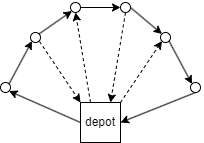
\includegraphics[width=\textwidth]{splitting_1.png}
        \caption{Merge}
    \end{subfigure}
    \begin{subfigure}[t]{0.24\textwidth}
        \centering
        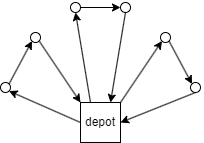
\includegraphics[width=\textwidth]{splitting_2.png}
        \caption{Split}
    \end{subfigure}
    \caption{Merge-Split operator}
\end{figure}

\subsubsection{Genetic Algorithm}

The genetic algorithm is used to maintain a population of diverse solutions and to guide the search process.
\begin{algorithm}
    \caption{Genetic Algorithm}
    \KwIn{A population $P$}
    \KwOut{A new population $P'$}
    $P' \leftarrow P$\;
    $s_{best} \leftarrow \text{BestSolution}(P)$\;
    \ForEach{$s \in P'$}{
        $s, s^* \leftarrow \text{SimulatedAnnealing}(s, T, \alpha)$\;
        $s_{best} \leftarrow \text{BestSolution}(s^*, s_{best})$\;
    }
    $P' \leftarrow P \cup P' \cup \{s_{best}\}$\;
    $P'.sort()$\;
    $P' \leftarrow P'[0:|P|]$\;
    \Return{$P'$}
\end{algorithm}

We modify the genetic algorithm to select the best individuals from the parent population, offspring population, and the best solution encountered during the simulated annealing process.
This is because the simulated annealing process may generate a better solution than the parent population and offspring population, as mentioned earlier.

\section{Experiments}
\label{sec:experiments}

\subsection{Setup}

We first experiment the proposed algorithm with different population sizes and cooling rates.
Since smaller instances are easier to solve and show little difference in results, we use a relatively large $egl$-S1-A dataset for this experiment.
The best set of parameters is selected for the subsequent experiments.

We then test the proposed Genetic Simulated Annealing Algorithm (GSA) on the benchmark instances of the $gdb$, $egl$, and $val$ datasets.
The $gdb$ dataset contains the smallest instances, then the $val$ dataset, and the $egl$ dataset contains the largest instances.
This allows us to evaluate the robustness of the algorithm on different scales of the problem.

The algorithm is implemented in Python and run on a computer with an Intel Core i9-12900H CPU and 16GB of RAM.
The environment is Ubuntu 22.04.3 LTS with Python 3.9.7.
For each instance, we conduct 5 independent runs with a runtime limit of 60 seconds.
The random seed is set to 1, 2, 3, 4, and 5 for each run, respectively.

\subsection{Results}

The results of the first experiment are shown in Table \ref{tab:pop and cooling}.
The table shows the average cost of the solutions found by the algorithm.
\begin{table}[h]
    \centering
    \begin{tabular}{ccc}
        \toprule
        Population Size & Cooling Rate & Avg Cost\\
        \midrule
        5 & 0.999 & 5170.2 \\
        10 & 0.999 & 5223.6 \\
        20 & 0.999 & 5199.8 \\
        5 & 0.99 & 5226 \\
        10 & 0.99 & 5184.2 \\
        20 & 0.99 & 5203.4 \\
        \bottomrule
    \end{tabular}
    \caption{Results of different population sizes and cooling rates on the $egl$-S1-A dataset}
    \label{tab:pop and cooling}
\end{table}

The results of the second experiment is shown in Table \ref{tab:gdb}, \ref{tab:val}, and \ref{tab:egl}.
The table shows the cost of the best solution found by the algorithm and the average cost of the solutions.
We also incorporate the theoretical lower bound and result of MEANS \cite{MEANS} for comparison.
The columns labeled $Gap_1$ and $Gap_2$ show the percentage gap between the best solution found by the algorithm and the lower bound, and the result of MEANS, respectively.

\begin{table}[h]
    \centering
    \resizebox{\linewidth}{!}{
        \begin{tabular}{llllllll}
            \toprule
            \multirow{2}{*}{Dataset} & \multirow{2}{*}{Lower Bound} & \multicolumn{2}{c}{MEANS} & \multicolumn{2}{c}{GSA} & \multirow{2}{*}{$Gap_1$} & \multirow{2}{*}{$Gap_2$}\\
            & & Avg & Best & Avg & Best & & \\
            \midrule
            1     & 316      & 316     & 316      & 316      & 316      & 0        & 0        \\
            2     & 339      & 339     & 339      & 339      & 339      & 0        & 0        \\
            3     & 275      & 275     & 275      & 275      & 275      & 0        & 0        \\
            4     & 287      & 287     & 287      & 287      & 287      & 0        & 0        \\
            5     & 377      & 377     & 377      & 377      & 377      & 0        & 0        \\
            6     & 298      & 298     & 298      & 298      & 298      & 0        & 0        \\
            7     & 325      & 325     & 325      & 325      & 325      & 0        & 0        \\
            8     & 348      & 348.7   & 348      & 353.2    & 350      & 0.574713 & 0.574713 \\
            9     & 303      & 303     & 303      & 308      & 303      & 0        & 0        \\
            10    & 275      & 275     & 275      & 275      & 275      & 0        & 0        \\
            11    & 395      & 395     & 395      & 395      & 395      & 0        & 0        \\
            12    & 458      & 458     & 458      & 461.2    & 458      & 0        & 0        \\
            13    & 536      & 536     & 536      & 540.8    & 536      & 0        & 0        \\
            14    & 100      & 100     & 100      & 100      & 100      & 0        & 0        \\
            15    & 58       & 58      & 58       & 58       & 58       & 0        & 0        \\
            16    & 127      & 127     & 127      & 127      & 127      & 0        & 0        \\
            17    & 91       & 91      & 91       & 91       & 91       & 0        & 0        \\
            18    & 164      & 164     & 164      & 164      & 164      & 0        & 0        \\
            19    & 55       & 55      & 55       & 55       & 55       & 0        & 0        \\
            20    & 121      & 121     & 121      & 121      & 121      & 0        & 0        \\
            21    & 156      & 156     & 156      & 156      & 156      & 0        & 0        \\
            22    & 200      & 200     & 200      & 200      & 200      & 0        & 0        \\
            23    & 233      & 233     & 233      & 234.6    & 233      & 0        & 0        \\
            Avg      & 253.7826 & 253.813 & 253.7826 & 254.6435 & 253.8696 & 0.034264 & 0.034264 \\
            No. best & -        & 22      & 23       & 18       & 22       & -        & -        \\
            \bottomrule
        \end{tabular}
    }
    \caption{Results on the $gdb$ dataset}
    \label{tab:gdb}
\end{table}

\begin{table}[h]
    \centering
    \resizebox{\linewidth}{!}{
        \begin{tabular}{llllllll}
            \toprule
            \multirow{2}{*}{Dataset} & \multirow{2}{*}{Lower Bound} & \multicolumn{2}{c}{MEANS} & \multicolumn{2}{c}{GSA} & \multirow{2}{*}{$Gap_1$} & \multirow{2}{*}{$Gap_2$}\\
            & & Avg & Best & Avg & Best & & \\
            \midrule
            1A    & 173      & 173      & 173      & 174.4    & 173      & 0        & 0        \\
            1B    & 173      & 173      & 173      & 175.4    & 173      & 0        & 0        \\
            1C    & 245      & 245      & 245      & 246.4    & 245      & 0        & 0        \\
            2A    & 227      & 227      & 227      & 227      & 227      & 0        & 0        \\
            2B    & 259      & 259      & 259      & 261      & 260      & 0.3861   & 0.3861   \\
            2C    & 457      & 457.2    & 457      & 471.4    & 469      & 2.625821 & 2.625821 \\
            3A    & 81       & 81       & 81       & 81.2     & 81       & 0        & 0        \\
            3B    & 87       & 87       & 87       & 87.2     & 87       & 0        & 0        \\
            3C    & 138      & 138      & 138      & 138.2    & 138      & 0        & 0        \\
            4A    & 400      & 400      & 400      & 405.6    & 400      & 0        & 0        \\
            4B    & 412      & 412      & 412      & 416.8    & 412      & 0        & 0        \\
            4C    & 428      & 431.1    & 428      & 442      & 434      & 1.401869 & 1.401869 \\
            4D    & 526      & 532.9    & 530      & 545.8    & 540      & 2.661597 & 1.886792 \\
            5A    & 423      & 423      & 423      & 423      & 423      & 0        & 0        \\
            5B    & 446      & 446      & 446      & 446.6    & 446      & 0        & 0        \\
            5C    & 473      & 474      & 474      & 474      & 474      & 0.211416 & 0        \\
            5D    & 573      & 582.9    & 577      & 600.4    & 597      & 4.188482 & 3.466205 \\
            6A    & 223      & 223      & 223      & 223.4    & 223      & 0        & 0        \\
            6B    & 233      & 233      & 233      & 238.2    & 233      & 0        & 0        \\
            6C    & 317      & 317      & 317      & 318.6    & 317      & 0        & 0        \\
            7A    & 279      & 279      & 279      & 285.2    & 279      & 0        & 0        \\
            7B    & 283      & 283      & 283      & 284      & 283      & 0        & 0        \\
            7C    & 334      & 334      & 334      & 340.4    & 336      & 0.598802 & 0.598802 \\
            8A    & 386      & 386      & 386      & 387.2    & 386      & 0        & 0        \\
            8B    & 395      & 395      & 395      & 395      & 395      & 0        & 0        \\
            8C    & 518      & 525.9    & 521      & 538.6    & 537      & 3.667954 & 3.071017 \\
            9A    & 323      & 323      & 323      & 328.8    & 326      & 0.928793 & 0.928793 \\
            9B    & 326      & 326      & 326      & 328      & 326      & 0        & 0        \\
            9C    & 332      & 332      & 332      & 335.2    & 332      & 0        & 0        \\
            9D    & 385      & 391      & 391      & 399.4    & 393      & 2.077922 & 0.511509 \\
            10A   & 428      & 428      & 428      & 432.2    & 429      & 0.233645 & 0.233645 \\
            10B   & 436      & 436      & 436      & 440.4    & 439      & 0.688073 & 0.688073 \\
            10C   & 446      & 446      & 446      & 449.8    & 446      & 0        & 0        \\
            10D   & 525      & 533.6    & 531      & 539.8    & 538      & 2.47619  & 1.318267 \\
            Avg      & 343.8235 & 345.1059 & 344.5294 & 349.4294 & 346.9706 & 0.915312 & 0.708554 \\
            No. best & -        & 26       & 28       & 3        & 21       & -        & -        \\
            \bottomrule
        \end{tabular}
    }
    \caption{Results on the $val$ dataset}
    \label{tab:val}
\end{table}

\begin{table}[h]
    \centering
    \resizebox{\linewidth}{!}{
        \begin{tabular}{llllllll}
            \toprule
            \multirow{2}{*}{Dataset} & \multirow{2}{*}{Lower Bound} & \multicolumn{2}{c}{MEANS} & \multicolumn{2}{c}{GSA} & \multirow{2}{*}{$Gap_1$} & \multirow{2}{*}{$Gap_2$}\\
            & & Avg & Best & Avg & Best & & \\
            \midrule
            E1-A & 3548     & 3548     & 3548     & 3585     & 3561     & 0.366404 & 0.366404 \\
            E1-B & 4498     & 4516.5   & 4498     & 4555     & 4543     & 1.000445 & 1.000445 \\
            E1-C & 5566     & 5601.6   & 5595     & 5703.8   & 5687     & 2.173913 & 1.644325 \\
            E2-A & 5018     & 5018     & 5018     & 5040.6   & 5027     & 0.179354 & 0.179354 \\
            E2-B & 6305     & 6341.4   & 6317     & 6450.8   & 6430     & 1.982554 & 1.788824 \\
            E2-C & 8243     & 8355.7   & 8335     & 8660.4   & 8615     & 4.51292  & 3.359328 \\
            E3-A & 5898     & 5898.8   & 5898     & 6031.4   & 5996     & 1.66158  & 1.66158  \\
            E3-B & 7704     & 7802.9   & 7775     & 7999.4   & 7946     & 3.141225 & 2.199357 \\
            E3-C & 10163    & 10321.9  & 10292    & 10534    & 10457    & 2.892847 & 1.603187 \\
            E4-A & 6408     & 6475.2   & 6456     & 6681.6   & 6658     & 3.901373 & 3.128872 \\
            E4-B & 8884     & 9023     & 8998     & 9409.6   & 9305     & 4.738856 & 3.411869 \\
            E4-C & 11427    & 11645.8  & 11561    & 12043.4  & 11859    & 3.78052  & 2.577632 \\
            S1-A & 5018     & 5039.8   & 5018     & 5206.2   & 5152     & 2.670387 & 2.670387 \\
            S1-B & 6384     & 6433.4   & 6388     & 6707     & 6689     & 4.777569 & 4.71196  \\
            S1-C & 8493     & 8518.3   & 8518     & 8736.4   & 8640     & 1.730837 & 1.432261 \\
            S2-A & 9824     & 9959.2   & 9895     & 10515    & 10397    & 5.832655 & 5.073269 \\
            S2-B & 12968    & 13231.6  & 13147    & 13896.2  & 13789    & 6.330969 & 4.883243 \\
            S2-C & 16353    & 16509.8  & 16430    & 17577.2  & 17408    & 6.451416 & 5.952526 \\
            S3-A & 10143    & 10312.7  & 10257    & 10932.6  & 10862    & 7.088633 & 5.898411 \\
            S3-B & 13616    & 13876.6  & 13749    & 14620.6  & 14463    & 6.220623 & 5.193105 \\
            S3-C & 17100    & 17305.8  & 17207    & 18452.6  & 18353    & 7.327485 & 6.66008  \\
            S4-A & 12143    & 12419.2  & 12341    & 13434    & 13123    & 8.070493 & 6.336602 \\
            S4-B & 16093    & 16441.2  & 16337    & 17626    & 17468    & 8.544087 & 6.922936 \\
            S4-C & 20375    & 20767.2  & 20538    & 22673    & 22531    & 10.5816  & 9.703963 \\
            Avg      & 9673.833 & 9806.817 & 9754.833 & 10294.66 & 10206.63 & 5.507555 & 4.631465 \\
            No. best & -        & 2        & 5        & 0        & 0        & -        & -        \\
            \bottomrule
        \end{tabular}
    }
    \caption{Results on the $egl$ dataset}
    \label{tab:egl}
\end{table}

\subsection{Analysis}

For the first experiment, we observe that a population size of 5 and a cooling rate of 0.999 yield the best results.
This is because a smaller population size allows the algorithm to run the simulated annealing process more times within the same time limit.
A higher cooling rate allows the algorithm to explore the solution space further.
This is consistent with the intuition that a higher cooling rate allows the algorithm to escape local minima more easily.

For the second experiment, we observe that the proposed Genetic Simulated Annealing Algorithm (GSA) performs well on the $gdb$ and $val$ datasets.
The algorithm finds the best solution for 22 out of 23 instances in the $gdb$ dataset and 21 out of 28 instances in the $val$ dataset.
And the average gap between the best solution found by GSA and the lower bound is less than 0.1\% for the $gdb$ dataset and less than 1\% for the $val$ dataset.
This indicates that the algorithm is effective in finding near-optimal solutions for small and medium-sized instances.

However, the algorithm struggles with the $egl$ dataset, which contains larger instances.
The average gap between the best solution found by GSA and the lower bound is around 5\%.
This suggests that the algorithm may require more sophisticated techniques or additional runtime to solve large instances effectively.

\section{Conclusion}
\label{sec:conclusion}

The proposed Genetic Simulated Annealing Algorithm (GSA) is a hybrid algorithm that combines simulated annealing and genetic algorithms.
The algorithm is effective in finding near-optimal solutions for small and medium-sized instances of the Capacitated Arc Routing Problem (CARP), showing a gap of less than 1\% between the best solution found by GSA and the lower bound for the $gdb$ and $val$ datasets.
However, the algorithm struggles with large instances, which suggests that more sophisticated techniques or additional runtime may be required to solve large instances effectively, with a gap of around 5\% for the $egl$ dataset.
The algorithm can be further improved by incorporating more advanced move operators, exploring different population initialization strategies, and tuning the parameters based on the characteristics of the instances.

\printbibliography

\end{document}
